\chapter{Main Chapter 1}
\label{chap: reactive transport model}
\fancyhead[R]{\uppercase{Chapter \thechapter. 
    Main Chapter 1
    }}
% \fancyhead[RE]{\rightmark}
% \fancyhead[LE, RO]{\thepage}
\begin{refsection}
% \linenumbers
\normalsize
% -------------------------------------------------------
%                    BEGIN MAIN TEXT
% -------------------------------------------------------

\section{Introduction}

This chapter comprises four parts. 

\section{Equation}
\label{sec:chap1: equation}
\subsection{Equation Example}
The equation example can be described as follows: 
\begin{equation}
    \pdv{t} \left( \varepsilon_{\mathrm{g}}\,\rho_{\mathrm{g}}\,Y_{\mathrm{g}}^{\ce{O3}} \right)
    + 
    \dots
    \label{eqn:chap1: equation example}
\end{equation}


\section{Figure}
\label{sec:chap1: Figure}
% figure: geometry and mesh of micro-reactor
\begin{figure}[!htbp]
    \centering
    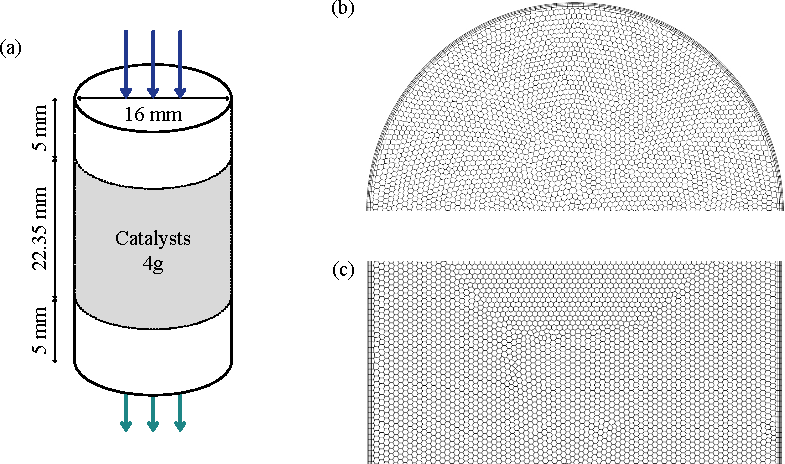
\includegraphics[width=.85\textwidth]{fig/chap_RxnMod-mesh_fixed_bed.pdf}
    \caption{Computational domain and mesh of the micro fixed-bed reactor}
    \label{fig:Chap1: mesh of micro-reactor}
\end{figure}

\autoref{fig:Chap1: mesh of micro-reactor} shows ...

\section{Table}
\label{sec:chap1: Table}

\autoref{tab:Chap1: Comparison} shows ... \autocite{liujs2016, wang2014catalytic}. 

\begin{table}[!h]
    \centering
    \vspace{10pt}
    \caption{Comparison of numerical results with experimental data}
    \begin{tabular}{cccccccc}
        \toprule
        Case & $C_{\mathrm{g,in}}^{\ce{O3}}$ & Packed $\varepsilon_{\mathrm{s}}$ & $U_{\mathrm{g}}$ & $k_\mathrm{r}$ & $C_{\mathrm{g,out}}^{\ce{O3}}$ & $ C_{\mathrm{g,out}}^{\ce{O3}}/C_{\mathrm{g,in}}^{\ce{O3}}$ & APE \\ 
        \midrule
        Unit & \si{ppmv} & - & \si{\m/\s} & \si{\per\s} & \si{ppmv} & - & \si{\percent} \\
        \midrule
        Exp. 1 $^{*}$ & 115.1 & 0.5 & 0.1124 & 4.12 & 50.70 & \num{0.44000} & - \\
        Num. 1 & 115.1 & 0.5 & 0.1124 & 4.12 & 50.84 & \num{0.44170} & 0.39 \\
        Exp. 2 $^{**}$ & 100.0 & 0.5 & 0.57 & 49.12 & 9.054 & \num{0.09054} & - \\
        Num. 2 & 100.0 & 0.5 & 0.57 & 49.12 & 9.049 & \num{0.09049} & 0.06 \\
        \bottomrule \\[-10pt]
        \multicolumn{8}{l}{\footnotesize{
            $^*$ Data from the work of \textcite{liujs2016}.}} \\
        \multicolumn{8}{l}{\footnotesize{
            $^{**}$ Data from the work of \textcite{wang2014catalytic}.}} 
    \end{tabular}
    \label{tab:Chap1: Comparison}
\end{table}

\section{Conclusions}
The present study involved 

% \processdelayedfloats % put figures here
% -------------------------------------------------------
%                    END MAIN TEXT
% -------------------------------------------------------
\pagebreak
\addcontentsline{toc}{section}{References}

\begin{spacing}{1.1}
    \printbibliography[heading=subbibliography]
\end{spacing}
\end{refsection}